%! Author = tstreule

\section{Optical Microscopy}
%%%%%%%%%%%%%%%%%%%%%%%%%%%%%%%%%%%%%%%%%%%%%%%%%%%%%%
%%%%%%%%%%%%%%%%%%%%%%%%%%%%%%%%%%%%%%%%%%%%%%%%%%%%%%
\subsection{Reflection and Refraction}
%
\formbox{Law of Reflection}{\theta\ped{inc} = \theta_2}
\formbox{Law of Refraction}{\frac{n\ped{inc}}{n_2} = \frac{\lambda_0/\lambda\ped{inc}}{\lambda_0/\lambda_2} = \frac{\sin\theta_2}{\sin\theta\ped{inc}}}
\quad for $\theta\ped{inc}<\theta_c$
\formula{Total reflection}{\sin\theta_c = n_2/n\ped{inc}}
\quad \textbf{always total} if $n\ped{inc}<n_2$

\formula{Paraxial approx.}{\theta \simeq \sin\theta \simeq \tan\theta, \;\;\; \theta\ll 1}
\formula{Thin lens approx.}{R \ll S_o,\,S_i}
\formbox{Lens makers formula}{\frac{1}{S_o} + \frac{1}{S_i} = \frac{1}{f} = \frac{n_\textrm{lens}-n}{n} \left( \frac{1}{R_1} - \frac{1}{R_2} \right)}
%%%%%%%%%%%%%%%%%%%%%%%%%%%%%%%%%%%%%%%%%%%%%%%%%%%%%%
\subsection{Ray Tracing}
%
%	\begin{itemize}
%		\item Rays passing \textbf{through the optical center} of a lens continue in a straight line
%		\item Rays traveling \textbf{parallel to the optical axis} pass through the focal point after refraction and vice versa
%		\item \textbf{Parallel rays} pass through the same point in the focal plane after refraction and vice versa
%	\end{itemize}
\begin{minipage}{\linewidth}
    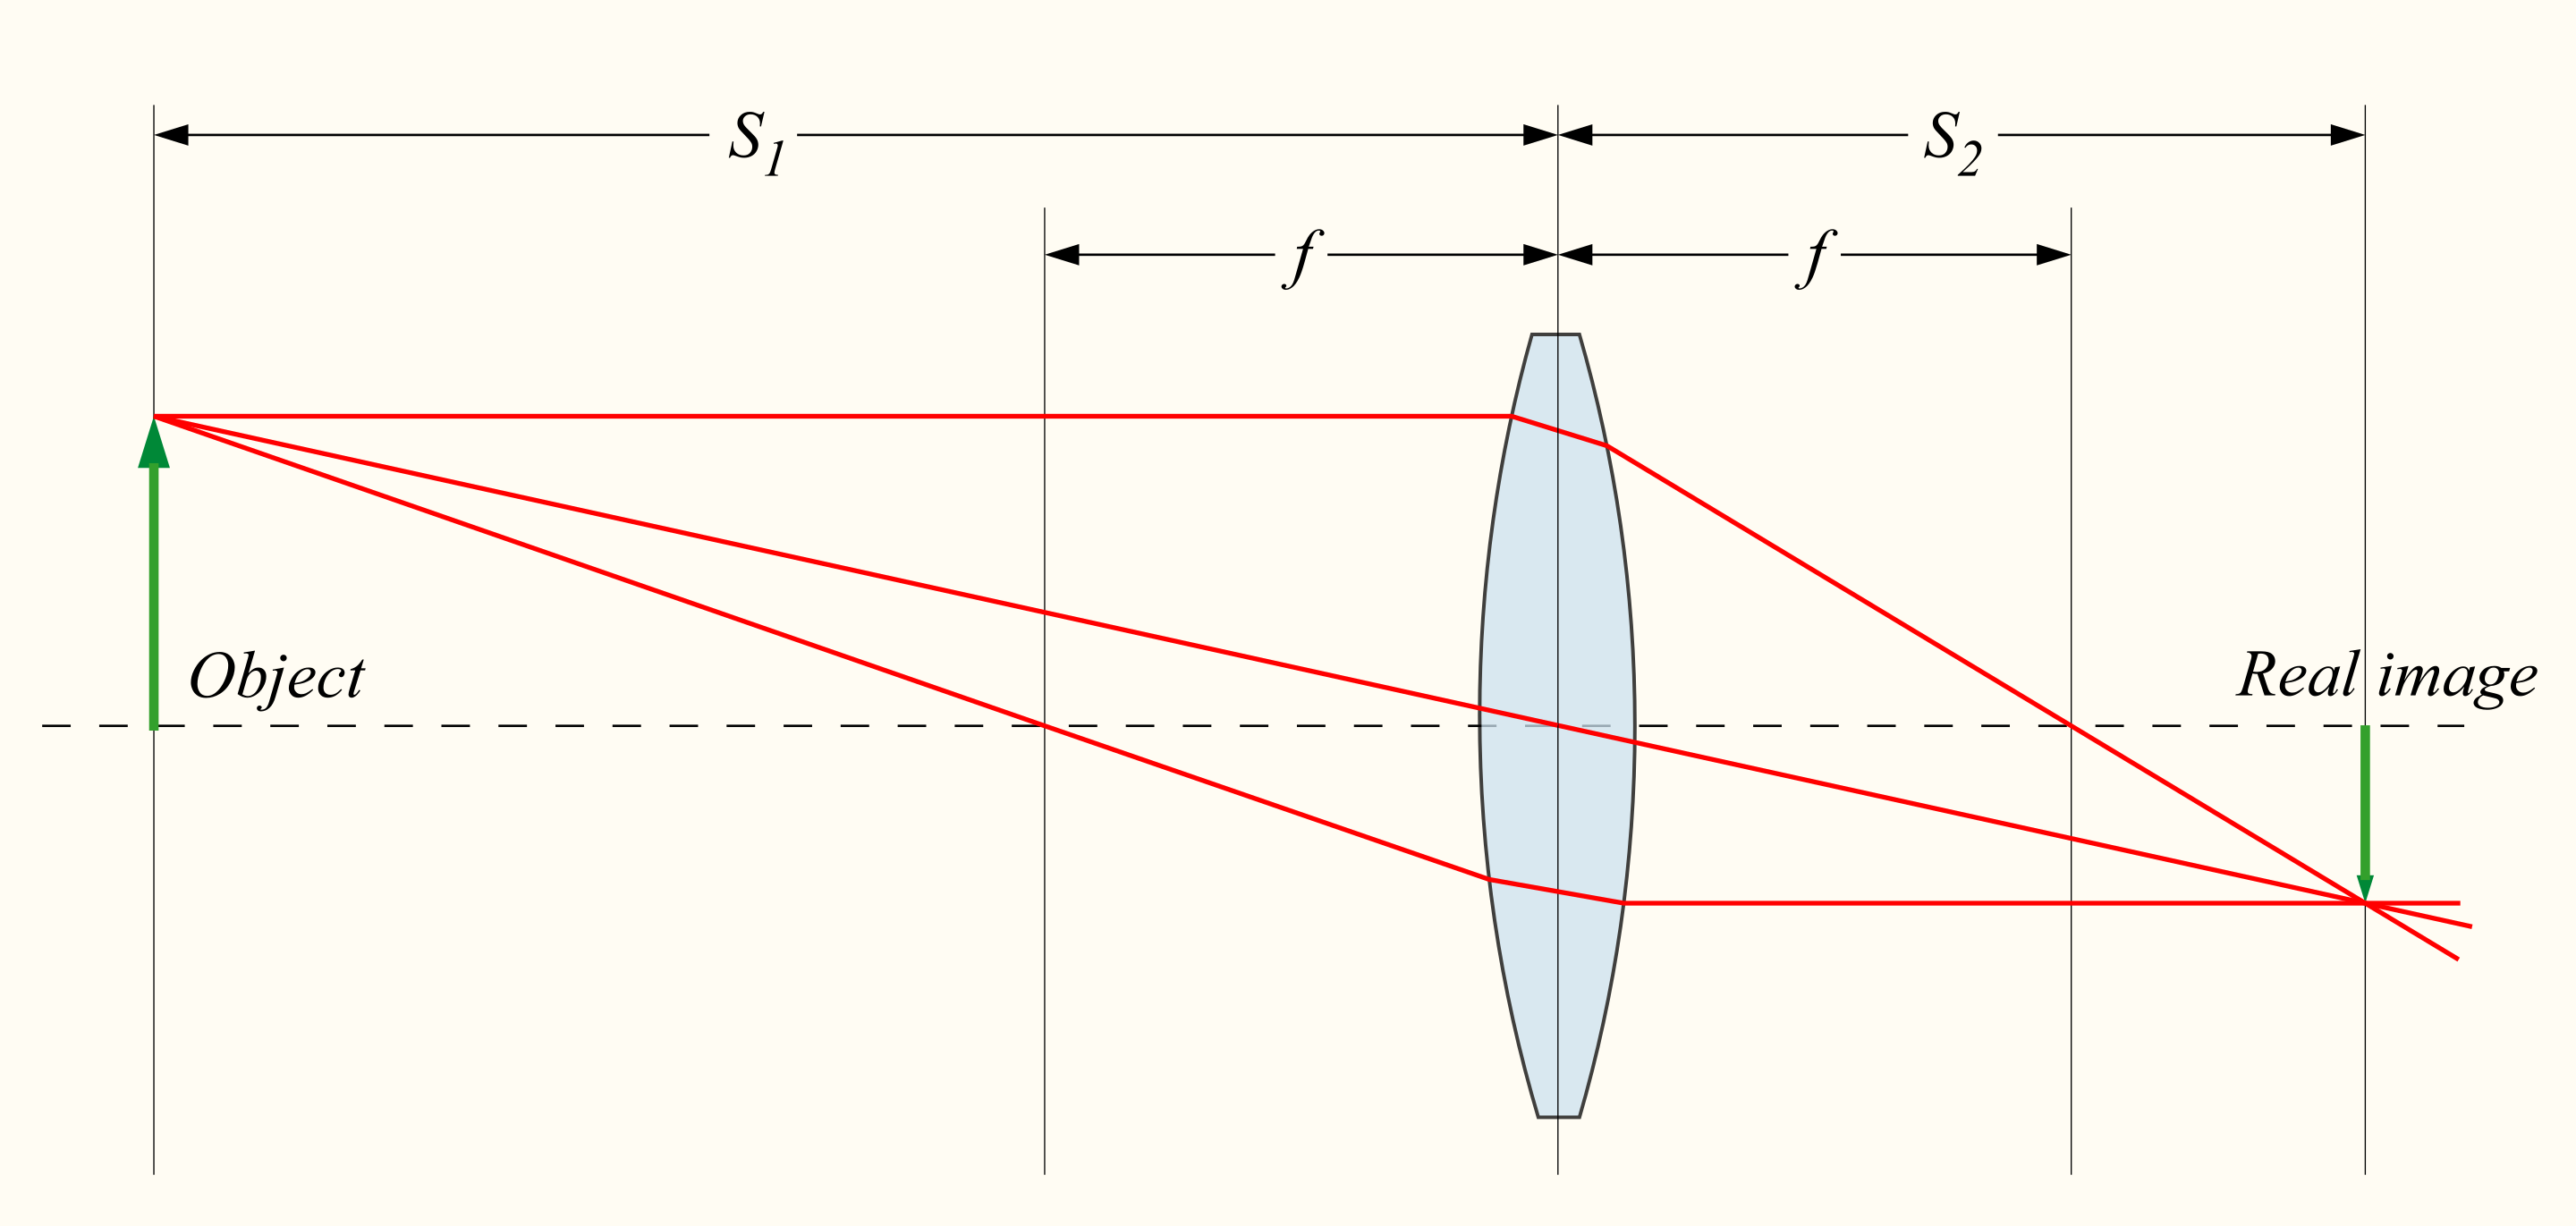
\includegraphics[width=.45\columnwidth]{Optical_Lens}
    \qquad
    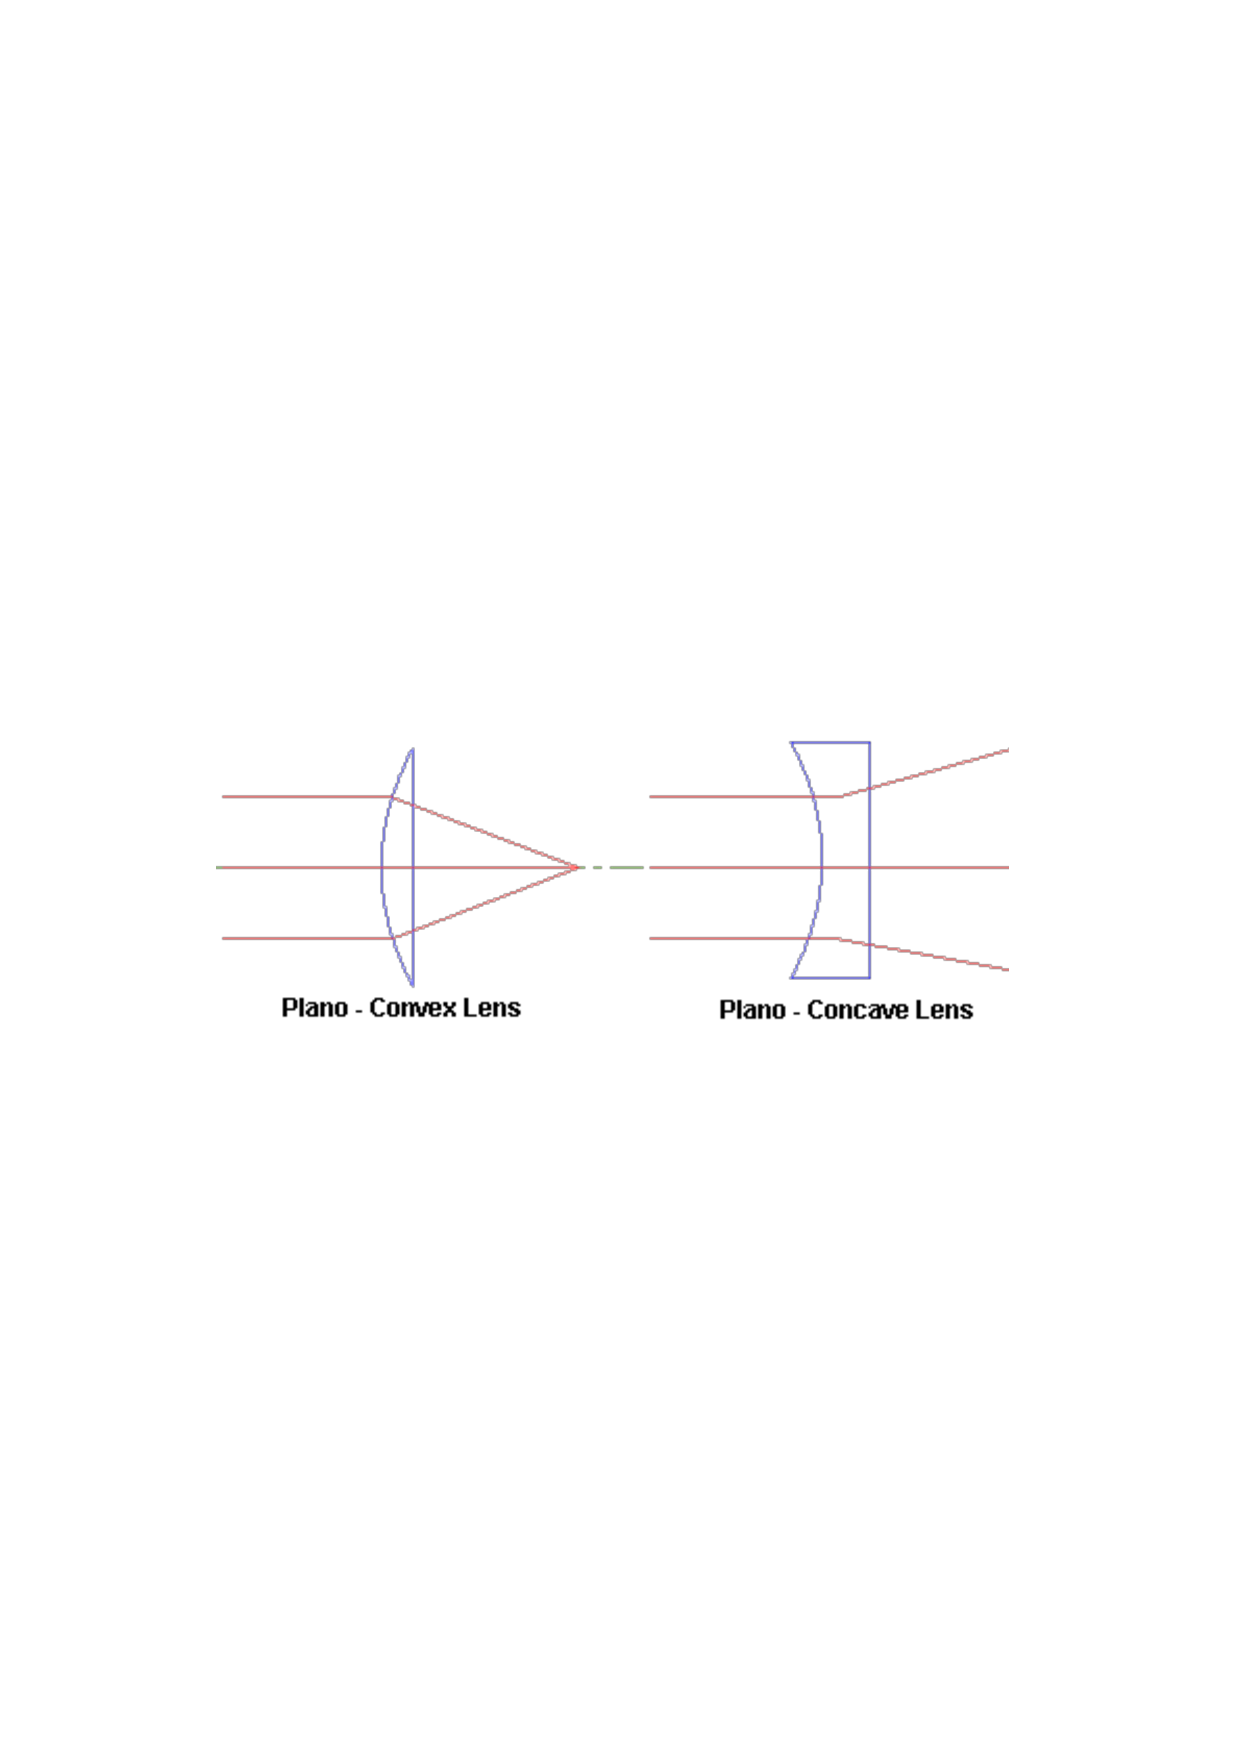
\includegraphics[width=.4\columnwidth]{Optical_Lens2}
\end{minipage}
%%%%%%%%%%%%%%%%%%%%%%%%%%%%%%%%%%%%%%%%%%%%%%%%%%%%%%
\begin{minipage}{\linewidth}
    \begin{minipage}[t]{.5\columnwidth-.5\columnsep}
        \subsubsection{Simple Microscope}
        %
        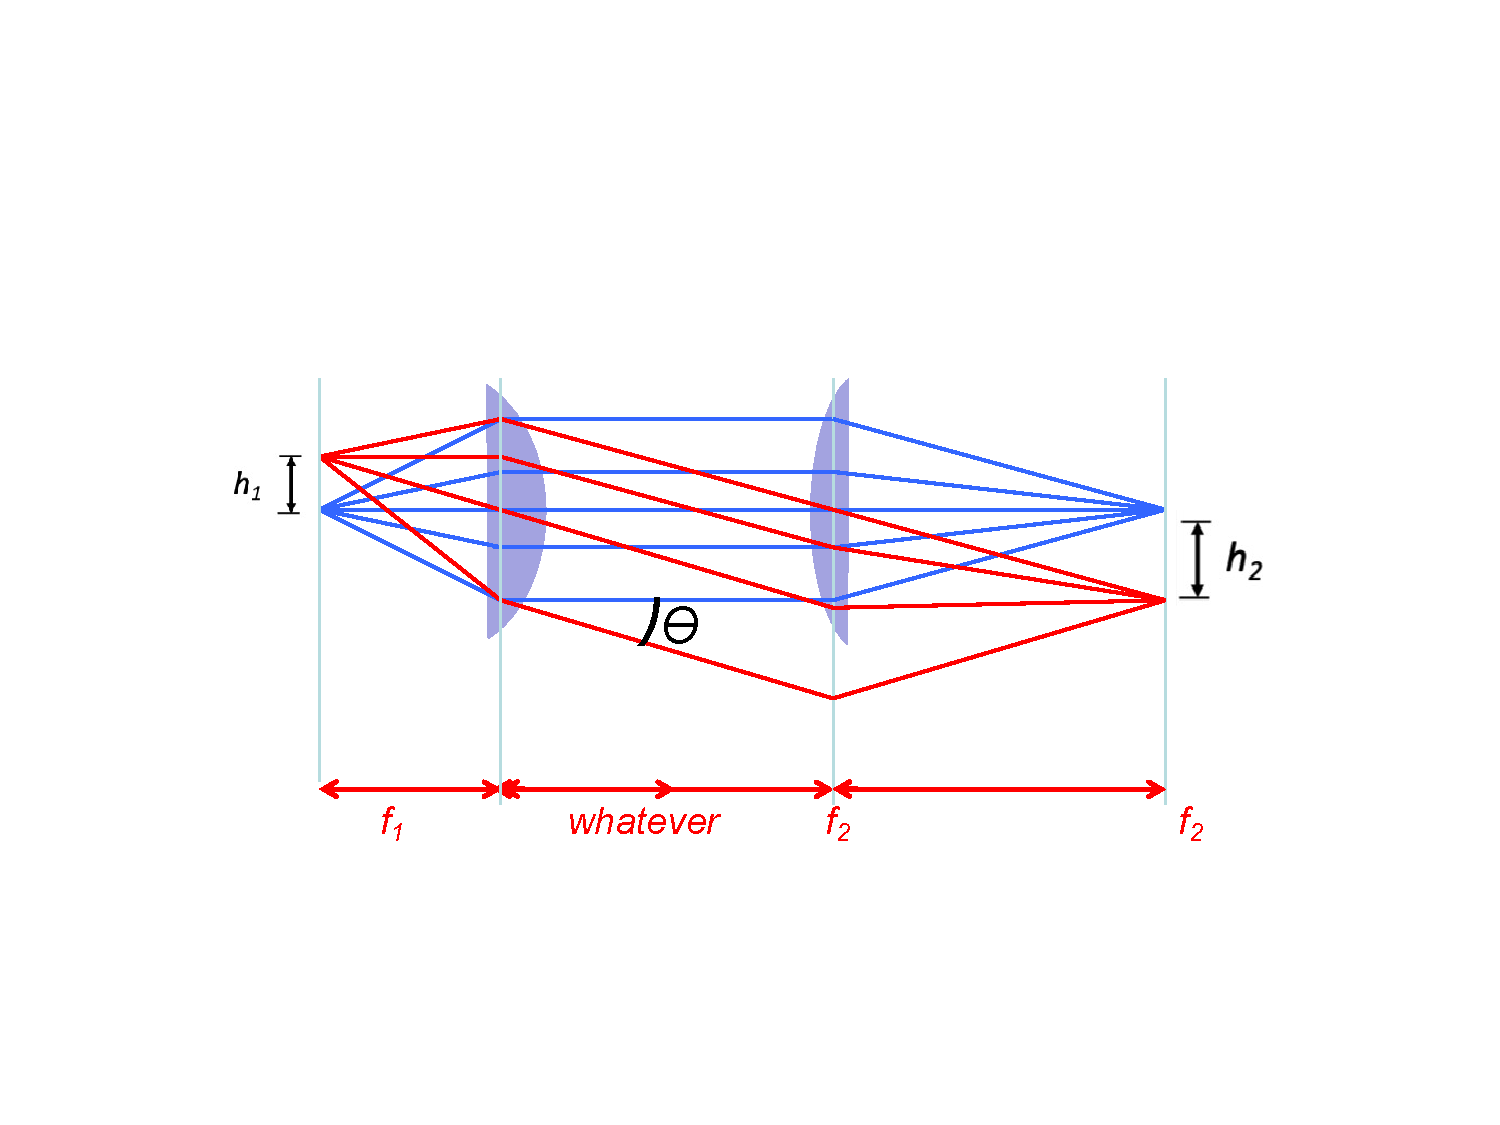
\includegraphics[width=\columnwidth]{Optical_Simple_Microscope}
    \end{minipage}%
    \hspace{\columnsep}%
    \begin{minipage}[t]{.5\columnwidth-.5\columnsep}
        \subsubsection{Beam Expander}
        %
        \hfill for light source

        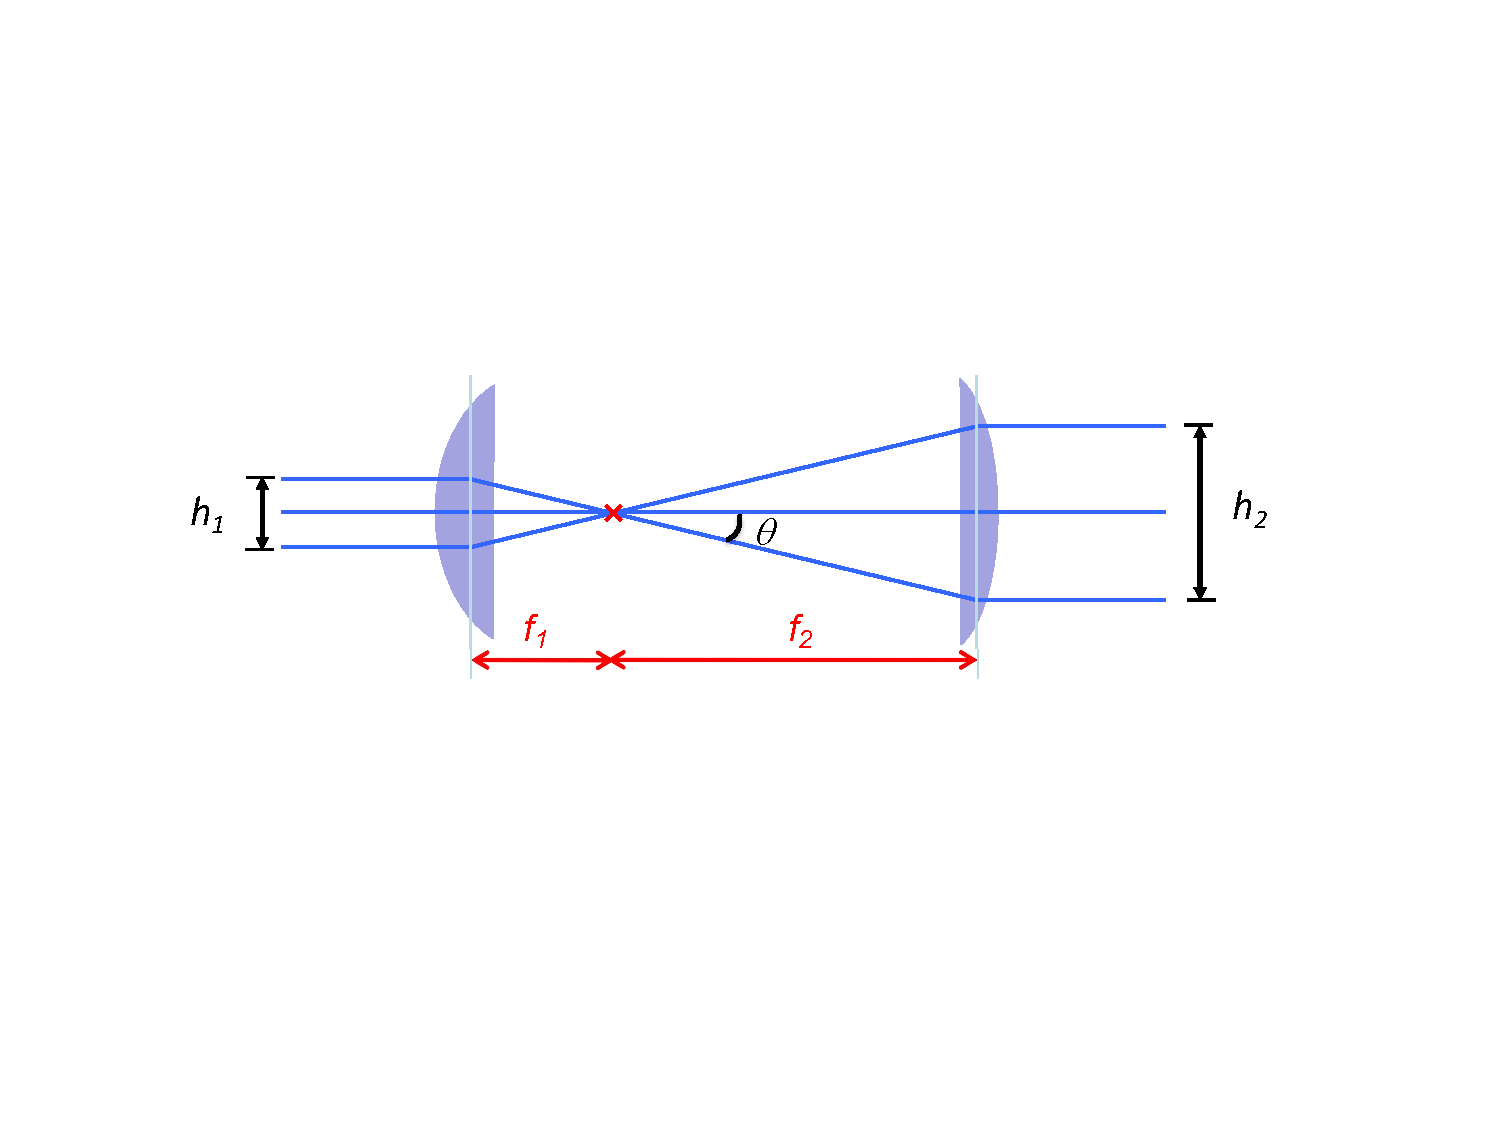
\includegraphics[width=\columnwidth]{Optical_Beam_Expander}
    \end{minipage}

    \formbox{Magnification}{M = h_2/h_1 \overset{*}{=} f_2/f_1}
    \quad * since $h_1 = f_1\sin\theta$
\end{minipage}
%%%%%%%%%%%%%%%%%%%%%%%%%%%%%%%%%%%%%%%%%%%%%%%%%%%%%%
\subsubsection{Simple ``modern'' Microscope}
%
\parbox{.5\columnwidth}{(uniform!) Illumination:}
\parbox{.5\columnwidth}{Camera: ($M = f_{tube} / f_{obj}$)}

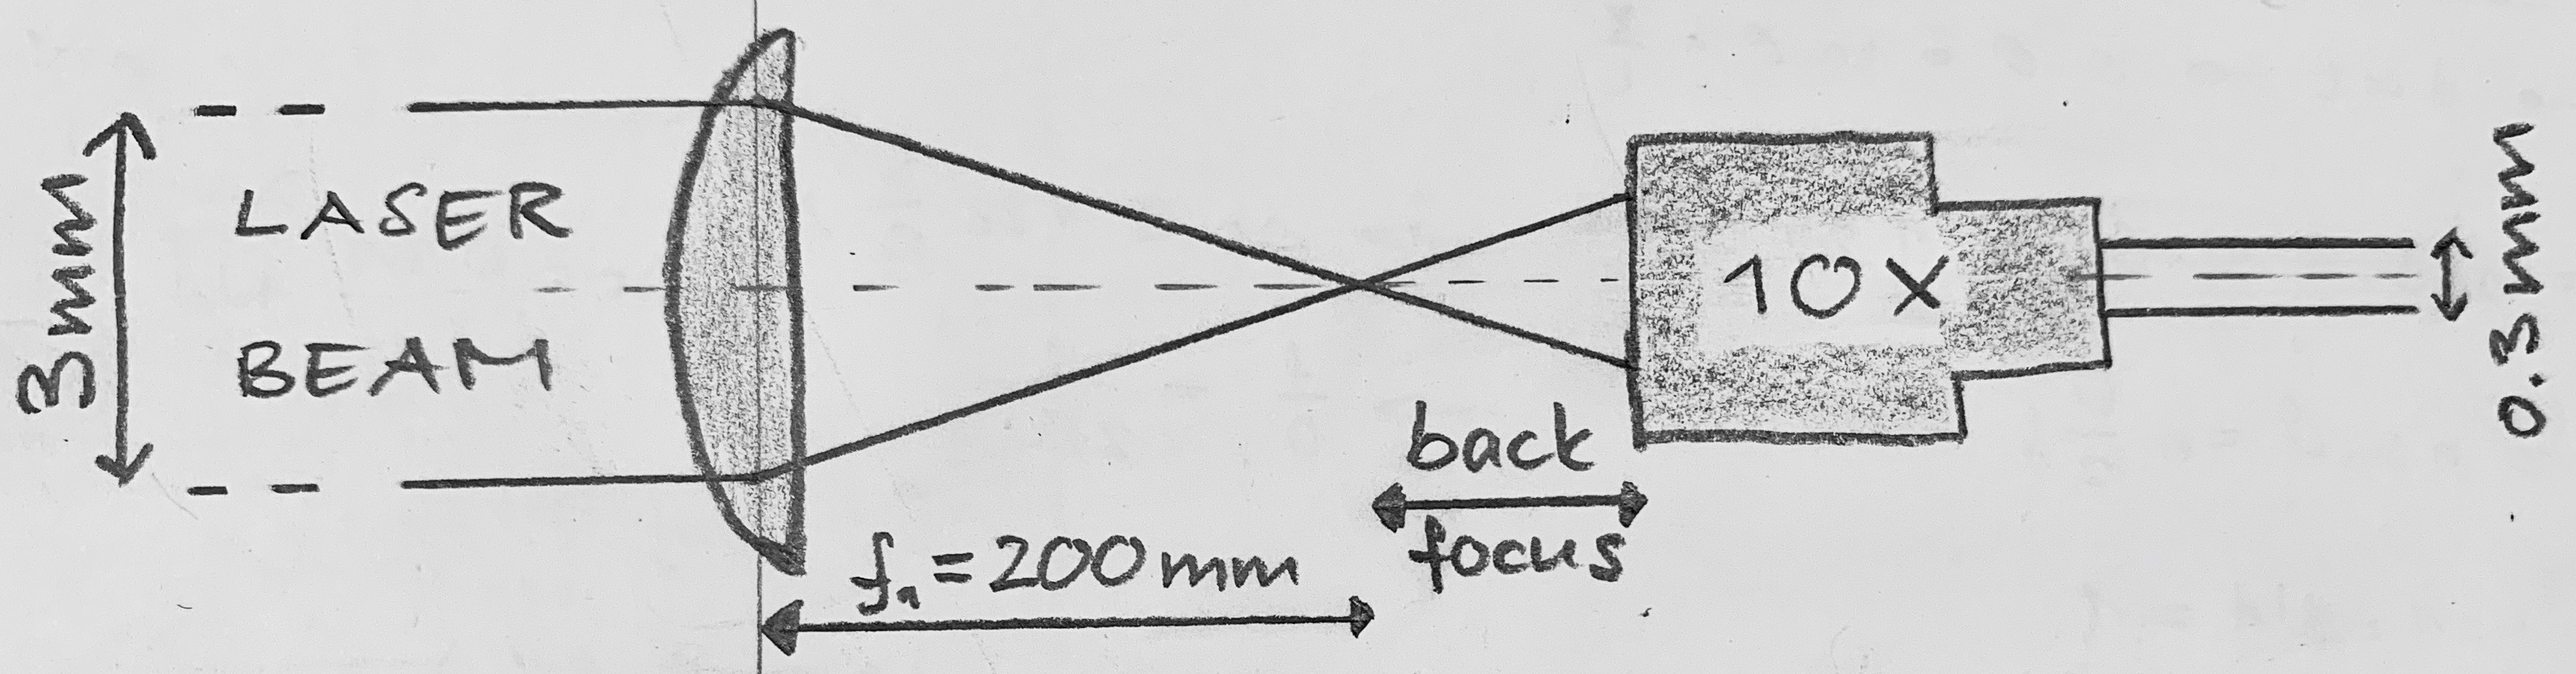
\includegraphics[width=.49\columnwidth]{Optical_Modern_Illumination}
\hfill
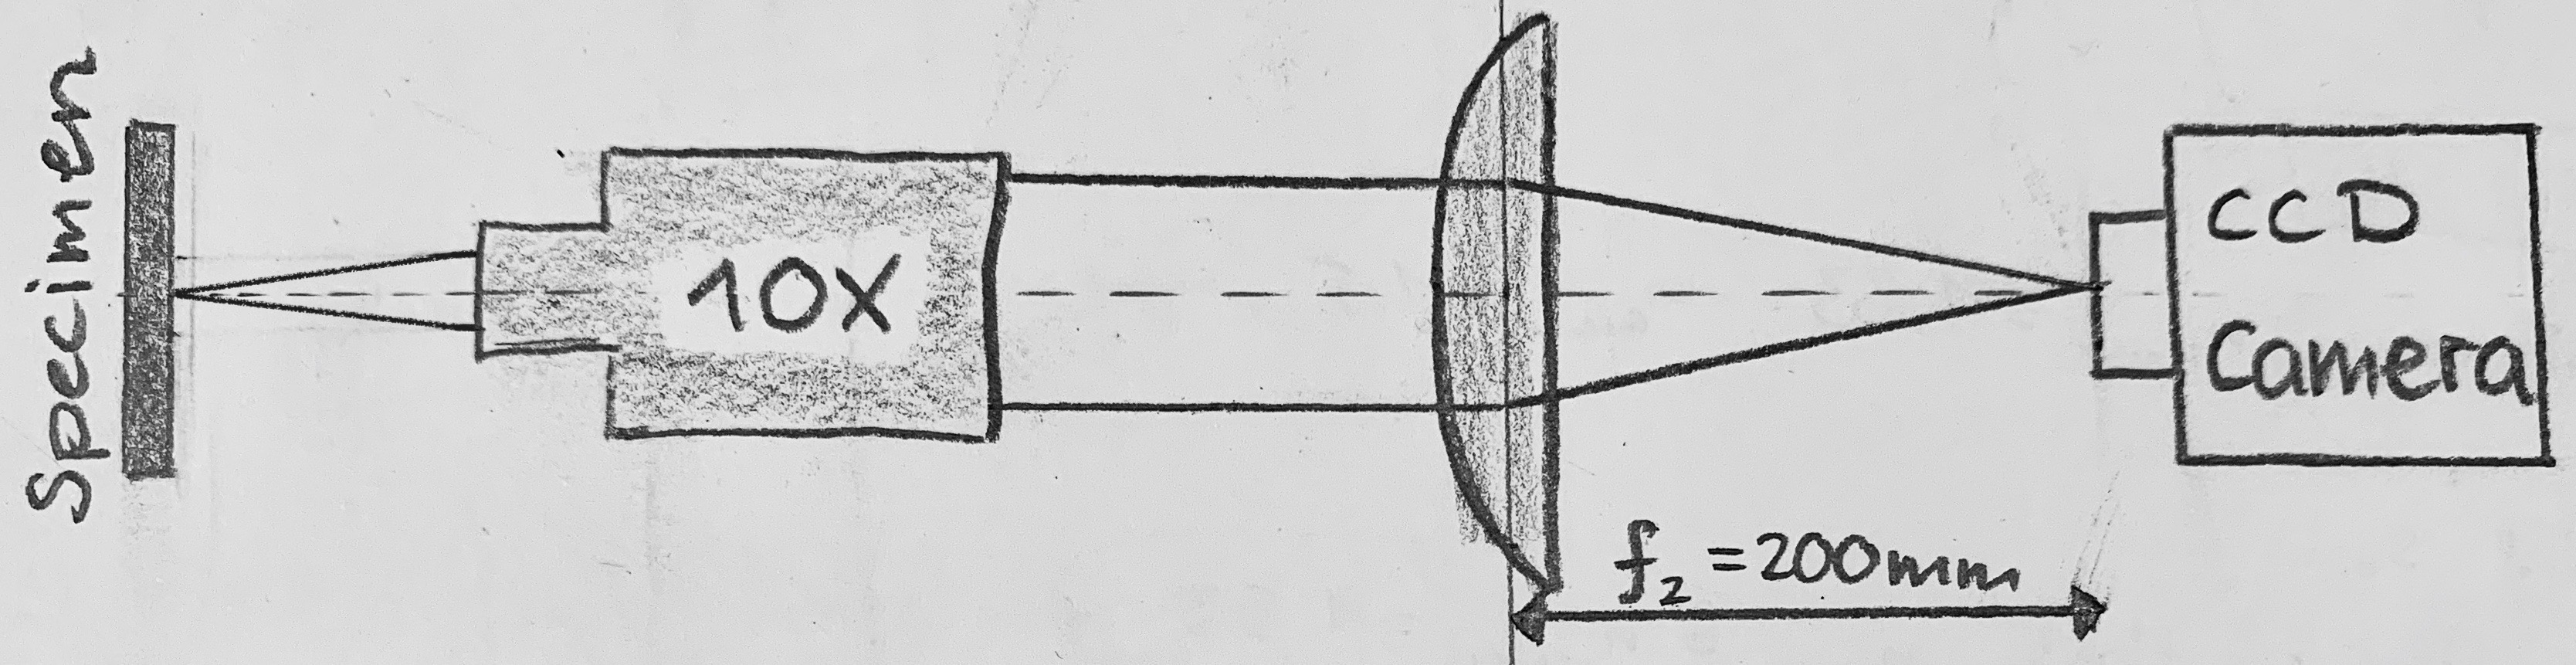
\includegraphics[width=.49\columnwidth]{Optical_Modern_Camera}

\parbox{.5\columnwidth}{\centering\small(Objective lens)}
\parbox{.5\columnwidth}{\centering\small(Tube lens)}
%%%%%%%%%%%%%%%%%%%%%%%%%%%%%%%%%%%%%%%%%%%%%%%%%%%%%%
\subsection{Fundamental Limits of Lenses \& Resulution}
%
Due to a \textbf{finite aperture} will points presented as the PSF (point-spread).

\begin{minipage}{.3\columnwidth}
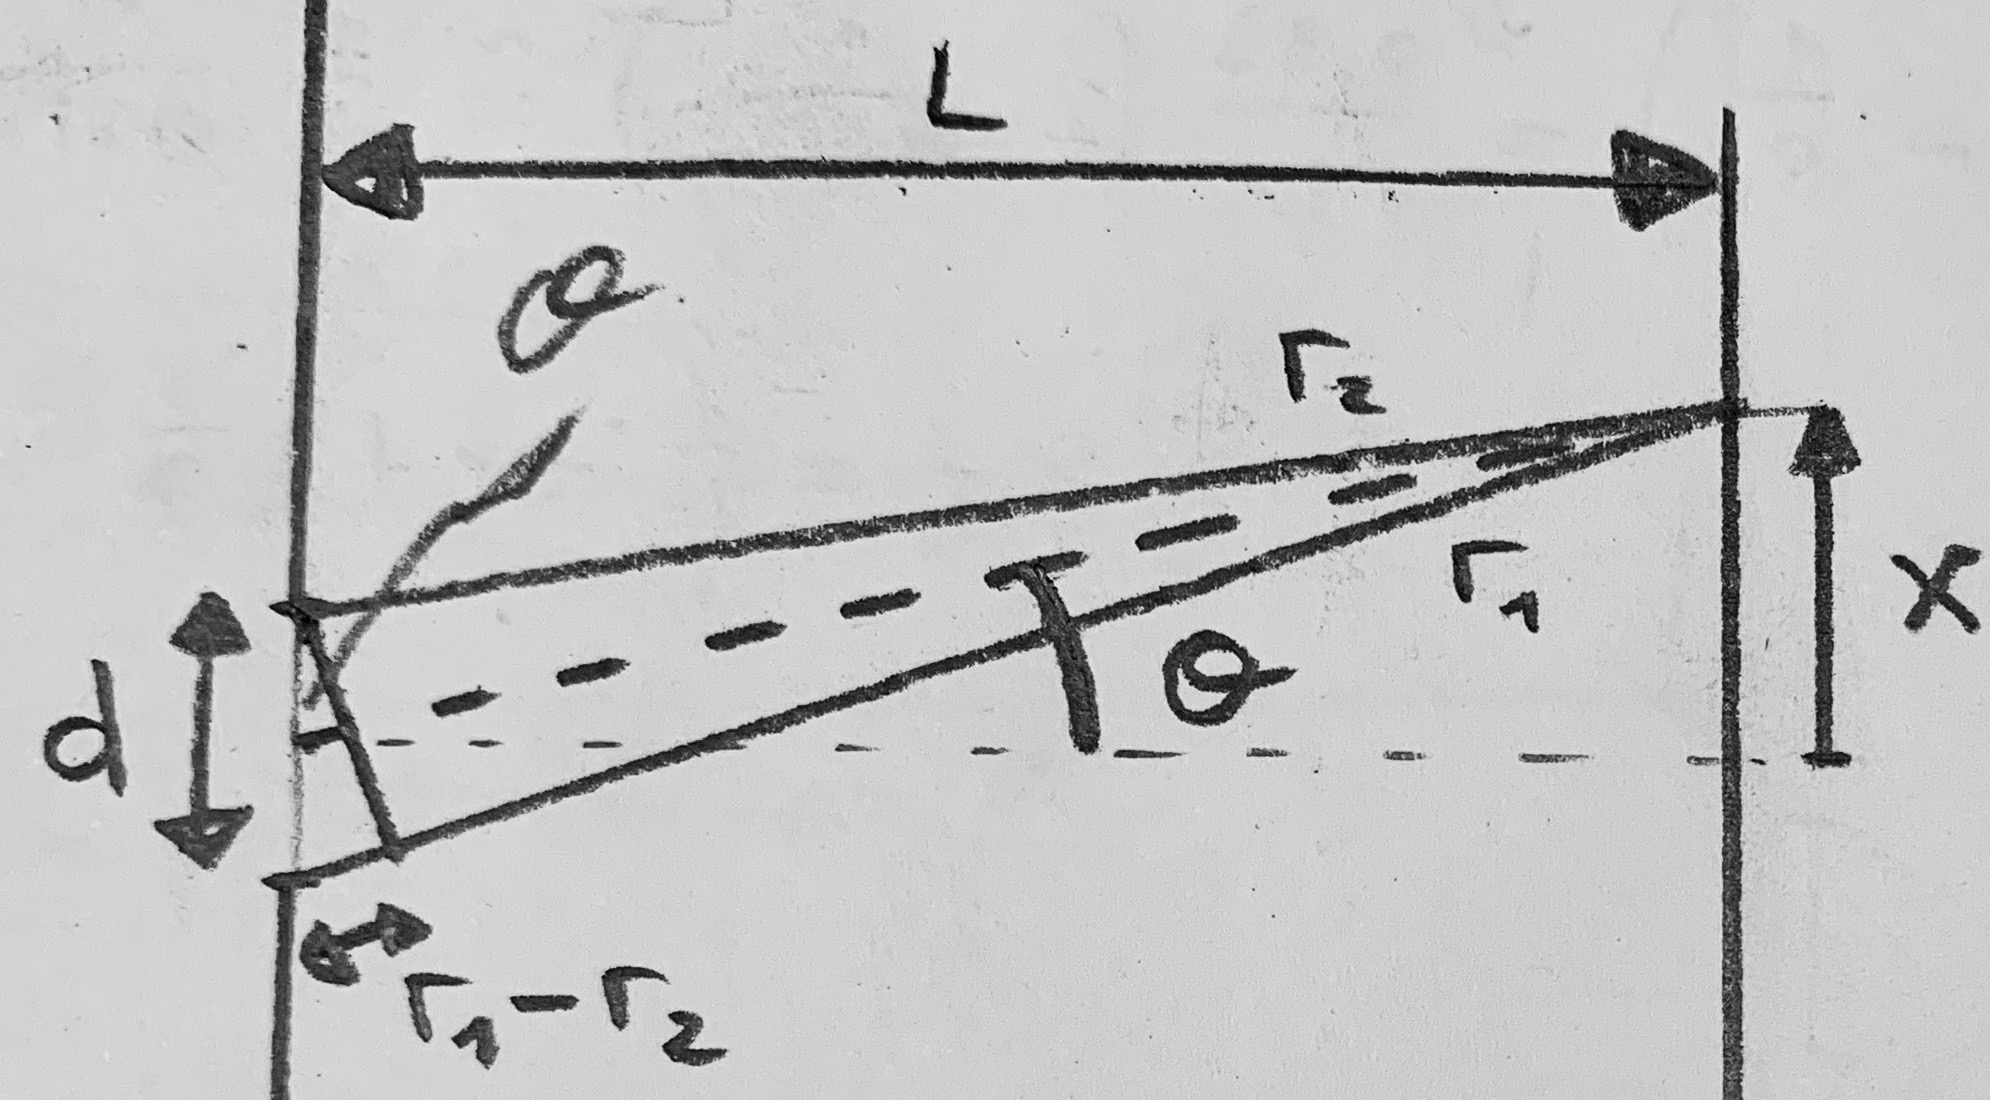
\includegraphics[width=\columnwidth]{Optical_PSF}
\end{minipage}%
\hspace{1.5\boxmargin}%
\begin{minipage}{.7\columnwidth-1.5\boxmargin}
First zero occurs at: \quad
$\theta \overset{(\theta\ll1)}{\simeq} \sin\theta \simeq 1.22\frac{\lambda_0}{d}$\\
$d$: radius of the aperture\par
$\bullet$ $\sin\theta \simeq \tan\theta = x/L$\\
$\bullet$ $r_1 - r_2 = d\cdot x/L$
\end{minipage}

\formtex{\textbf{Rayleigh criterion}}{maximum of the one is on the minimum of the}
\formtex{~}{other curve (FWHM)}
\formbox{Resolution}{\Delta r \simeq f\sin\theta \times M \simeq 1.22\frac{\lambda_0f}{D} \times M = 0.61\frac{\lambda_0n}{\textrm{NA}} \times M \vspace{-1mm}}
\formbox{Numerical Aperture}{\textrm{NA} = n\sin\theta \simeq n\,\frac{D}{2f}}
\quad $n$: refractive index,
\formula{~}{\text{$D$: aperture size of lens, $f$: focal length of lens}}
%%%%%%%%%%%%%%%%%%%%%%%%%%%%%%%%%%%%%%%%%%%%%%%%%%%%%%
\subsection{Fluorescence Microscopy}
%
Emitted photon has \textbf{less energy}.
$\to$ Absorption $\neq$ emission spectr.

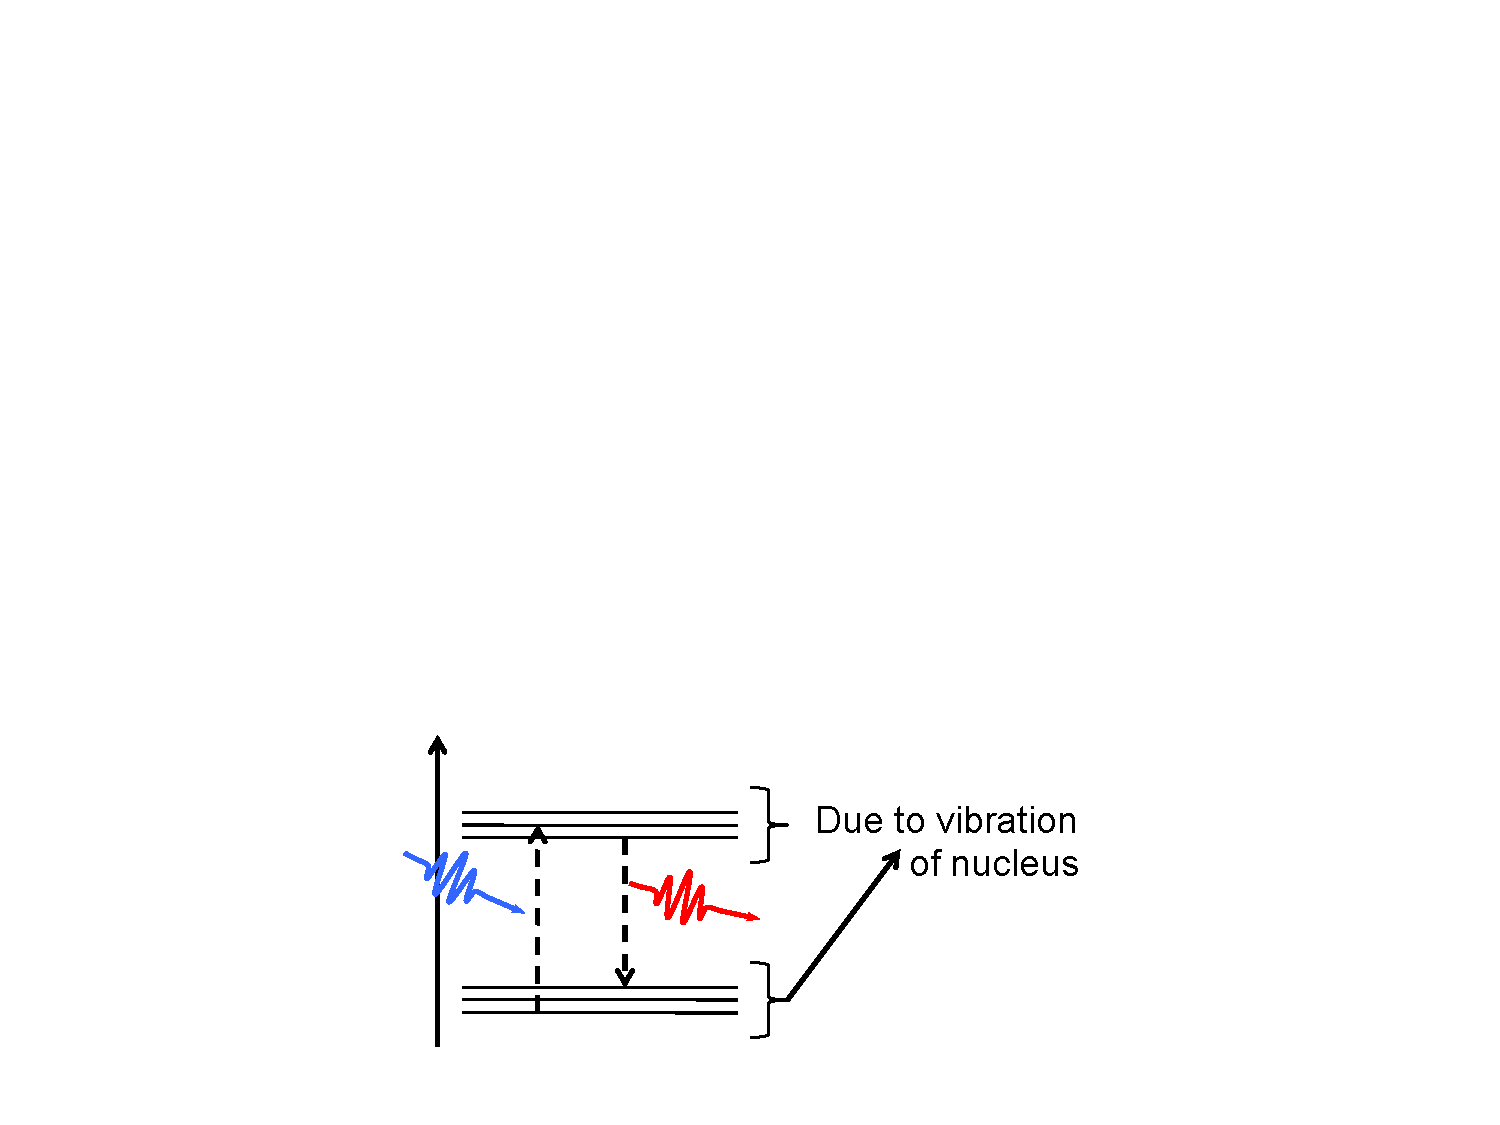
\includegraphics[width=.5\columnwidth]{Optical_Excitation_Emission}
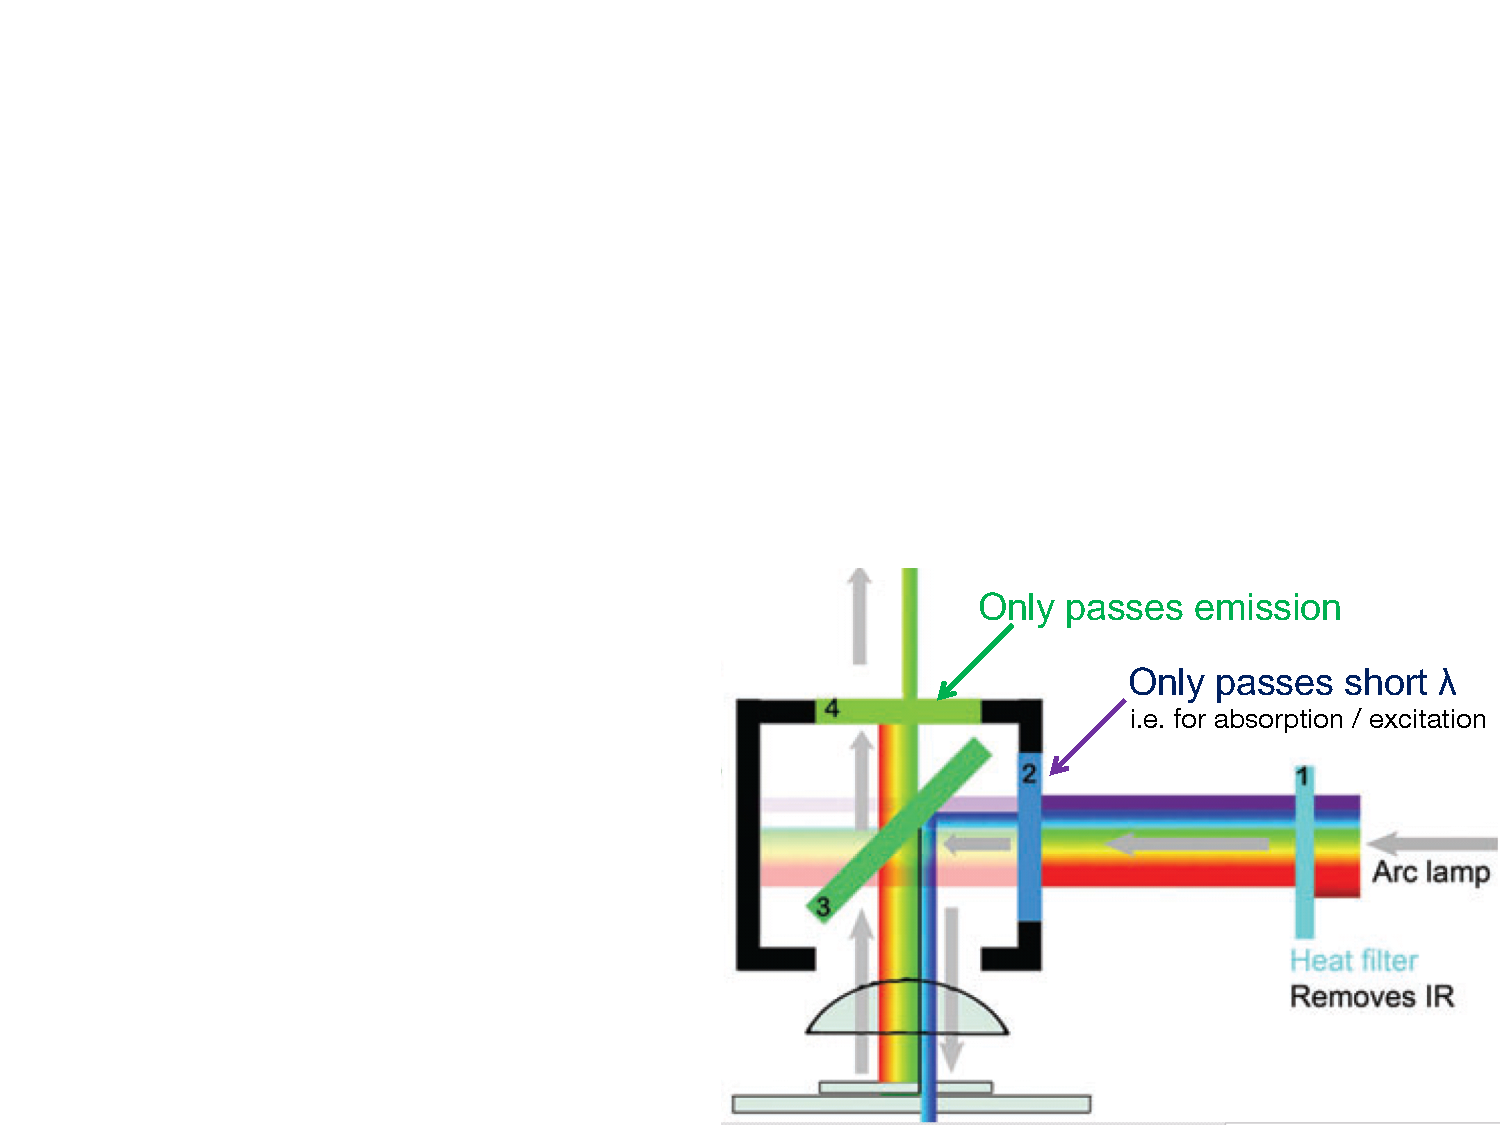
\includegraphics[width=.5\columnwidth]{Optical_Fluorescence_Setup}
